\documentclass[10pt]{article}
\usepackage[polish]{babel}
\usepackage[utf8]{inputenc}
\usepackage[T1]{fontenc}
\usepackage{graphicx}
\usepackage[export]{adjustbox}
\graphicspath{ {./images/} }
\usepackage{amsmath}
\usepackage{amsfonts}
\usepackage{amssymb}
\usepackage[version=4]{mhchem}
\usepackage{stmaryrd}

\title{Zestaw 4. }

\author{}
\date{}


\begin{document}
\maketitle
\begin{center}

\includegraphics[max width=\textwidth]{2024_11_21_4c68055ab3cf36522636g-1(1)}
\end{center}

\section*{GIMNAZJUM}
\begin{enumerate}
  \item Kwadrat o wymiarach 5 x 5 dzielimy na 25 identycznych małych kwadratów (rysunek poniżej). Ile wynosi suma kątów \(\angle P A Q, \angle P B Q, \angle P C Q, \angle P D Q, \angle P E Q\) ?\\
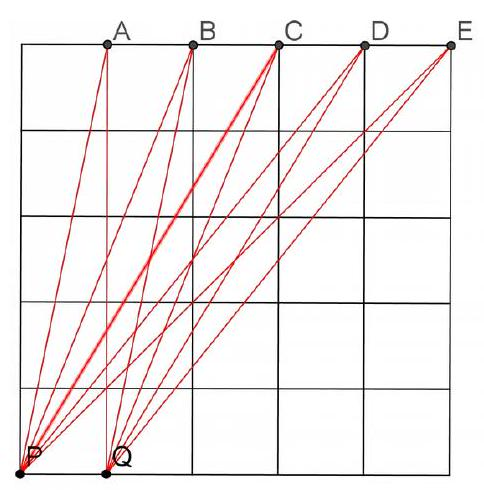
\includegraphics[max width=\textwidth, center]{2024_11_21_4c68055ab3cf36522636g-1}
  \item Ciąg Fibonacciego określony jest następująco:
\end{enumerate}

\[
F_{1}=F_{2}=1
\]

\[
F_{n+2}=F_{n+1}+F_{n} \text { dla } n \text { całkowitych dodatnich }
\]

Ustal, czy liczba \(F_{2015}\) jest parzysta.\\
3. Wyznacz wszystkie trójki liczb pierwszych \(p, q, r\) spełniające warunek:

\[
p \cdot q \cdot r=5(p+q+r)
\]

\section*{LICEUM}
\begin{enumerate}
  \item Dane są rozłączne okręgi \(o_{1}\) i \(o_{2}\) o środkach odpowiednio w punktach \(S\) i \(T\). Styczne do okręgu \(o_{2}\) poprowadzone z punktu \(S\) przecinają okrąg \(o_{1}\) w punktach \(A\) i \(B\). Styczne do okręgu \(o_{1}\) poprowadzone z punktu \(T\) przecinają okrąg \(o_{2}\) w punktach \(C\) i \(D\). Udowodnij, że odcinki \(A B\) i \(C D\) są równej długości.
  \item Ile wynosi odległość między środkami skośnych krawędzi czworościanu foremnego o krawędzi \(a\) ? (w czworościanie skośne krawędzie to te, które nie mają wspólnych końców).
  \item Znajdź wszystkie takie trójki liczb rzeczywistych \(a, b, c\), że
\end{enumerate}

\[
a+b+c=1
\]

oraz zachodzą równości:

\[
3(a+b c)=4(b+c a)=5(c+a b)
\]


\end{document}